\documentclass[letterpaper, 12pt]{article} %10pt por default
%\usepackage[paper=a4paper,left=24mm,right=24mm,top=20mm,bottom=20mm]{geometry}

\usepackage[utf8]{inputenc}
\usepackage[spanish]{babel}
\usepackage{geometry}
\usepackage{lipsum} %por si hay que hacer pruebas de como se ver\'ia
\usepackage{graphicx}
%\usepackage{rotating}
\usepackage{paracol}
\usepackage{multicol}
\usepackage{setspace}
\setstretch{1.2}
\setlength{\parskip}{16pt}
\usepackage{xstring}
\usepackage{xcolor}
\usepackage{xargs}
\usepackage{bbding} %para las palomitas
\usepackage{ragged2e}
\usepackage[hidelinks]{hyperref}
\usepackage{wrapfig}
\usepackage{lscape}
\usepackage{rotating}
\usepackage{epstopdf}
\usepackage{amsmath}
\usepackage{amssymb}
%\usepackage{caption}
%\usepackage{subcaption}
\usepackage{subfig}
%\usepackage[ruled,linesnumbered]{algorithm2e}
\usepackage{listings}
%\usepackage[toc, acronym]{glossaries}
\usepackage{verbatim}
%\usepackage{natbib}
\usepackage{float}
\usepackage{enumitem}
\usepackage{mathrsfs}
\usepackage{tcolorbox}
\usepackage[export]{adjustbox}
\usepackage[makeroom]{cancel}
\usepackage[firstpage=true]{background}
\usepackage[numbers]{natbib}

\usepackage{tikz}
\usetikzlibrary{positioning,shadows,backgrounds,automata,arrows,arrows.meta}
%\usetikzlibrary{arrows} %arrows meta
%\usepackage{tikz-qtree} % Easy tree drawing tool
%\tikzset{every tree node/.style={align=center,anchor=north}, level distance=2cm} % Configuration for q-trees


%\usepackage[breakable]{tcolorbox}



%Para estilo fancy
%\usepackage{fancyhdr}
%\usepackage{lastpage}fenter
%\pagestyle{fancy}
%\fancyhf{}

%\renewcommand{\headrulewidth}{0pt} %Quitar la l\'inea del encabezado de fancy
%\rfoot{\footnotesize{ P\'agina \thepage \hspace{1pt} de \pageref{LastPage} }}





\decimalpoint
%If you use either the babel or polyglossia package you'll have to change the name for the particular language
%you use with babel or polyglossia.
\addto\captionsspanish{% Replace "english" with the language you use
	\renewcommand{\contentsname}{Tabla de contenido}%
	\renewcommand{\listfigurename}{Lista de figuras}
	\renewcommand{\listtablename}{Lista de tablas}
	\renewcommand{\lstlistlistingname}{Lista de programas}
	\renewcommand{\glossaryname}{Glosario}
	% NOMBRES DE FIGURA, TABLA, ETC.
	%\renewcommand{\thefigure}{Fig.(\arabic{figure})}
	\renewcommand{\figurename}{Figura}
	%\renewcommand{\thetable}{Tab.(\arabic{table})}
	\renewcommand{\tablename}{Tabla}
	%\renewcommand{\theequation}{Eq.(\arabic{equation})}
	\renewcommand{\lstlistingname}{Programa}
}
% RENOMBRAR BIBLIOGRAF\'IA
%\renewcommand{\bibname}{\section{Referencias}}
%\renewcommand{\theenumi}{\Alph{enumi}}
\newcommand{\reftab}[1]{Tab.(\ref{#1})}
\newcommand{\reffig}[1]{Fig.(\ref{#1})}
\newcommand{\refeq}[1]{Ec.(\ref{#1})}
\newcommand{\refexp}[1]{Exp.(\ref{#1})}
\newcommand{\refdef}[1]{Def.(\ref{#1})}
\newcommand{\refsec}[1]{Sec.(\ref{#1})}
\newcommand{\refssec}[1]{Subsec.(\ref{#1})}
\newcommand{\refej}[1]{Ej.(\ref{#1})}
\newcommand{\refprog}[1]{Prog.(\ref{#1})}


% SIEMRPE EXISTIR\'A UNA CARPETA IMG
\graphicspath{{./img/}}

% ESPACIO ENTRE COLUMNAS DE MULTICOL
\setlength{\columnsep}{1cm}

% CONFIGURACI\'ON DE HIPERV\'INCULOS
%\hypersetup{
%    colorlinks=true,
%    linkcolor=black,
%    urlcolor=magenta
%}

% TAMA\~NO DE LA HOJA
\geometry{
	%headsep= 0pt,
	%head=0pt,
	%ignoreall,
	hmargin= {2.5cm, 2.5
		cm}, %izquierda, derecha
	vmargin= {2.5cm, 2.5cm} %arriba, abajo
}


% PREGUNTA Y RESPUESTA (pregunta dentro de itemizador)
\newcommand{\preg}[1][Pregunta]{
 \item \textbf{#1} \\
}
\newcommand{\resp}[1][Respuesta]{
 \textit{#1} \ \\
}

% ELEMENTO LIBRE DE ITEMIZADOR
\newcommand{\itemlibre}[1]{
 \tab - #1. \\
}

% CONCEPTO DE GLOSARIO: 1->llave, 2->concepto, 3->descripcion
% Requiere libreria glossaries
\newcommand{\itemg}[2]{
 \item \textbf{#1} #2 
 
 \enter
 
}

% ESPACIADORES
\newcommand{\enter}{\vspace{0.5cm}}
\newcommand{\tab}{\hspace{1cm}}

% L\'INEA PARA LLENADO (param: medida de la l\'inea en mm)
\newcommand{\sublinea}[1]{
 \rule{#1mm}{0.1mm}
<}

% LEYENDAS DE IMAGEN ALTERADAS A CURSIVA
\newcommand{\captionit}[1]{
    \caption{\textit{#1}}
}
\newcommand{\subcaptionit}[1]{
    \subcaption{\textit{#1}}
}

% CUADRO DE REMARCACI\'ON
\newenvironment{remark}[1]{
	\begin{tcolorbox}[
		colback= myNaranja!25,
		colframe= blue254!75,
		title=#1,
		arc= 3mm,
		sharp corners= northwest
	]
		\fontfamily{gag}\selectfont
}{\end{tcolorbox}}

\newcounter{cteorema}
\newenvironment{theo}[1]{
	\addtocounter{cteorema}{1}
	\begin{tcolorbox}[
		colback=orange!5,
		colframe=blue!50!black,
		title= \textbf{Teorema \thesection.\arabic{cteorema}. #1},
		arc= 3mm,
		sharp corners= north
		]
		\fontfamily{gag}\selectfont
}{\end{tcolorbox}}

\newcounter{cejemplo}
\newenvironment{ejem}[1]{
	\refstepcounter{cejemplo}
	\begin{tcolorbox}[
		breakable,
		colback=blue!5,
		colframe=blue!75!black,
		title= \textbf{Ejemplo \arabic{cejemplo}. #1},
		arc= 3mm,
		sharp corners= all
		]
		\fontfamily{gag}\selectfont
}{\end{tcolorbox}}

\newcounter{cdefinicion}
\newenvironment{defon}[1]{
	\addtocounter{cdefinicion}{1}
	\begin{tcolorbox}[
		colback=orange!20,
		colframe=blue254!75,
		title= \textbf{Definici\'on \thesection.\arabic{cdefinicion}. #1},
		arc= 3mm,
		sharp corners= west
		%breakable,
		%enhanced
		]
		\fontfamily{gag}\selectfont
	}{\end{tcolorbox}}



% CONVERSI\'ON DE CONTADORES A GLOBALES
%Para hacer global el contador de figura y no se repita al hacer un paracol
\globalcounter{figure}
\globalcounter{equation}








% COLORES DE PORTADA
\definecolor{myAzul}{HTML}{234ECA}
\definecolor{blue254}{HTML}{02528F}
\definecolor{myVerde}{HTML}{36A736}
\definecolor{myNaranja}{HTML}{FF4312}
\definecolor{guinda}{HTML}{660000}
\definecolor{azul}{HTML}{1A079F}
\definecolor{negro}{HTML}{000000}
\definecolor{blanco}{HTML}{FFFFFF}
\definecolor{dorado}{HTML}{996515}
\definecolor{ududff}{rgb}{0.30196078431372547,0.30196078431372547,1}
\definecolor{template_blue}{HTML}{003473}   % Color of Leiden University logo (Lei-Blauw)
\definecolor{subtitle}{cmyk}{0,0,0,0}       % Color for subtitle (white)
\definecolor{template_text}{HTML}{434655}   % Color for text
\definecolor{template_lightgrey}{HTML}{A8AABC}  % Color of the chapter banner   


% BORRAR SANGR\'IA EN GENERAL
\setlength\parindent{0pt}

% ALINEAR A LA DERECHA LOS N\'UMEROS DE FOOTNOTE
%\footnotemargin{\@makefnmark\hss}




% ESTILO PARA LISTINGS
\definecolor{codegreen}{rgb}{0,0.6,0}
\definecolor{codegray}{rgb}{0.5,0.5,0.5}
\definecolor{codepurple}{rgb}{0.58,0,0.82}
\definecolor{backcolour}{rgb}{0.95,0.95,0.92}

\lstdefinestyle{mystyle}{
	backgroundcolor=\color{backcolour},   
	commentstyle=\color{codegreen},
	keywordstyle=\color{blue},
	numberstyle=\tiny\color{codegray},
	stringstyle=\color{codepurple},
	basicstyle=\ttfamily\footnotesize,
	breakatwhitespace=false,         
	breaklines=true,                 
	captionpos=b,                    
	keepspaces=true,                 
	numbers=left,                    
	numbersep=5pt,                  
	showspaces=false,                
	showstringspaces=false,
	showtabs=false,                  
	tabsize=1
}

\lstset{style=mystyle}




\makeatletter
\newcommand\binomialCoefficient[2]{%
	% Store values 
	\c@pgf@counta=#1% n
	\c@pgf@countb=#2% k
	%
	% Take advantage of symmetry if k > n - k
	\c@pgf@countc=\c@pgf@counta%
	\advance\c@pgf@countc by-\c@pgf@countb%
	\ifnum\c@pgf@countb>\c@pgf@countc%
	\c@pgf@countb=\c@pgf@countc%
	\fi%
	%
	% Recursively compute the coefficients
	\c@pgf@countc=1% will hold the result
	\c@pgf@countd=0% counter
	\pgfmathloop% c -> c*(n-i)/(i+1) for i=0,...,k-1
	\ifnum\c@pgf@countd<\c@pgf@countb%
	\multiply\c@pgf@countc by\c@pgf@counta%
	\advance\c@pgf@counta by-1%
	\advance\c@pgf@countd by1%
	\divide\c@pgf@countc by\c@pgf@countd%
	\repeatpgfmathloop%
	\the\c@pgf@countc%
}
\makeatother



\newcommand{\pnormal}[3]{
	\backgroundsetup{
		scale=1,
		opacity= 0.05,
		angle= 0,
		contents= {
			
\includegraphics[width=0.75\paperwidth, height=0.9\paperheight]{../ImgPortada/IPN_Logo.png}
		}
	}
	\BgThispage
	\begin{center}
   		\begin{figure}[!tbp]
   			\centering
   			\subfloat{
\includegraphics[scale=0.2]{../ImgPortada/CIC_Logo.png}}
   			\hfill
   			\subfloat{
\includegraphics[scale=0.2]{../ImgPortada/MICROSE_Logo.png}}
   		\end{figure}
        
        {\LARGE \textcolor{guinda}{\textbf{I}nstituto \textbf{P}olit\'ecnico \textbf{N}acional} }
        \\ \vspace{1cm}
        {\LARGE \textit{ \textcolor{azul}{Centro de Investigaci\'on en Computaci\'on} } }
		\\
        {\Large \textit{ \textcolor{azul}{(\textbf{CIC})} } }
        \\ \vspace{2.5cm}
        {\Large \textsc{\underline{#1}}} %%%%%%%%%%Materia%%%%%%%%%%
        \\ \vspace{3cm}
        {\LARGE \textbf{ \textcolor{guinda}{#2} } } %%%%%%%%%%Título%%%%%%%%%%
        \\ \vspace{3cm}
        {\Large \textsc{ #3 } } %%%%%%%%%%Profesor%%%%%%%%%%
        \\ \vspace{2cm}
        {\Large \textsc{ Ing. Ricardo Aldair Tirado Torres } }
        %\ \\
        %A230720
        \\ \vspace{2cm}
        {\large \textsc{  \textsl{ Ciudad de M\'exico, \today } } }
    \end{center}
}




\begin{document}
	\pagenumbering{gobble}
	\pnormal
	{Lenguajes de descripción de hardware}
	{Práctica 5. Máquina de estados finitos.}
	{M. en C. Osvaldo Espinoza Sosa}
	\tableofcontents
	
	\pagenumbering{arabic}
	\newpage \section{Descripción estructural de un multiplexor \label{sec:s1}}

\begin{center}
	\begin{minipage}{12cm}
		\begin{tcolorbox}[title=Actividad 1]
			Capturar el código para describir en forma estructural el multiplexor en el lenguaje de su elección. Instanciar el módulo o componente que se encuentre en el mismo archivo. Simular el multiplexor.
		\end{tcolorbox}	
	\end{minipage}
\end{center}

La visualización RTL del multiplexor, usando descripción estructural en Verilog, se muestra en la \autoref{fig:mux_str_des_rtl}. La implementación se hace con la instanciación de un multiplexor, denominado ``MyMux'', visualizado en el interior del módulo (Ver \autoref{fig:mux_str_des_rtl2}). Las simulaciones se visualizan en la \autoref{fig:mux_str_des_wave}, en donde se muestra que el multiplexor descrito opera de manera correcta.

En los Anexos se localiza la descripción en Verilog de este multiplexor. En el código se tienen dos módulos, siendo el primero, el de la jerarquía más alta y en donde se realiza la declaración de las entradas y la salida, para luego instanciar al módulo llamado ``MyMux'' con la etiqueta ``u0''. Cabe señalar que los argumentos de la instancia se deben colocar en el orden correcto. El segundo módulo unicamente es la descripción de un multiplexor sencillo, utilizando el operador condicional ``?''.

\begin{figure}[ht]
	\centering
	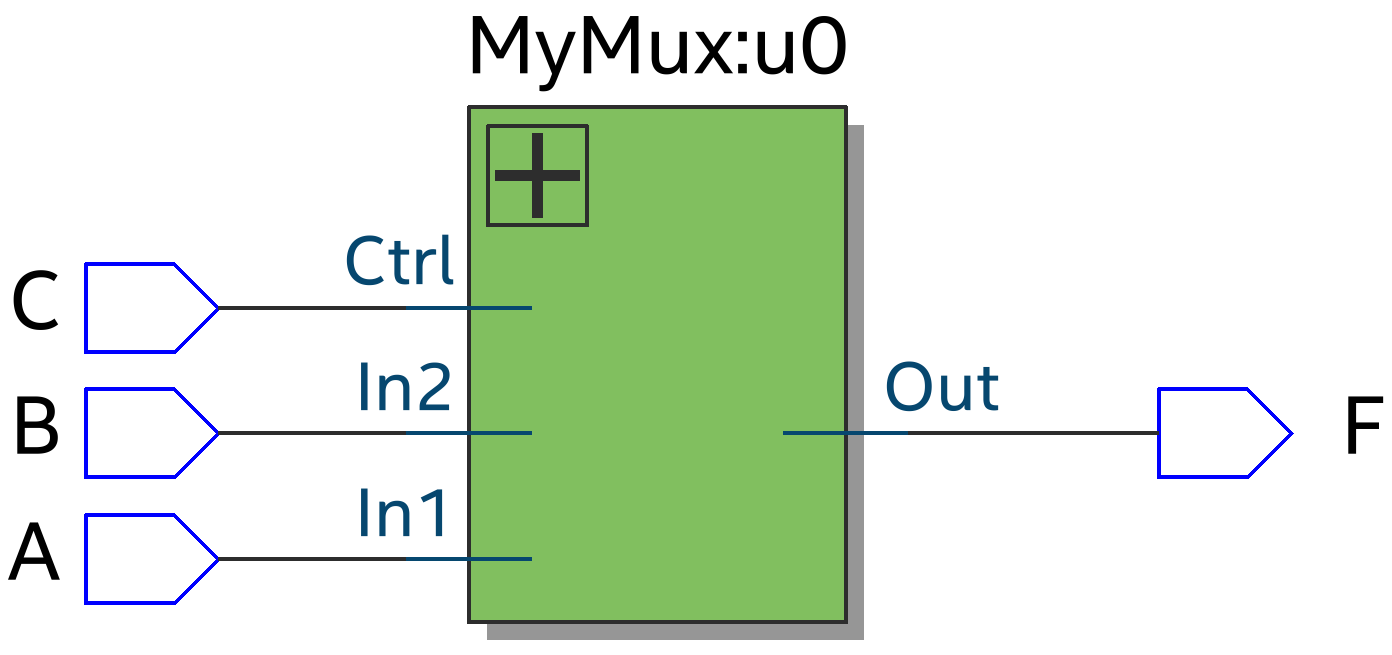
\includegraphics[scale=0.45]{Mux_Structural_Description_RTL.png}
	\caption{Diagrama RTL del multiplexor, descrito en forma estructural en Verilog. \label{fig:mux_str_des_rtl}}
\end{figure}

\begin{figure}[ht]
	\centering
	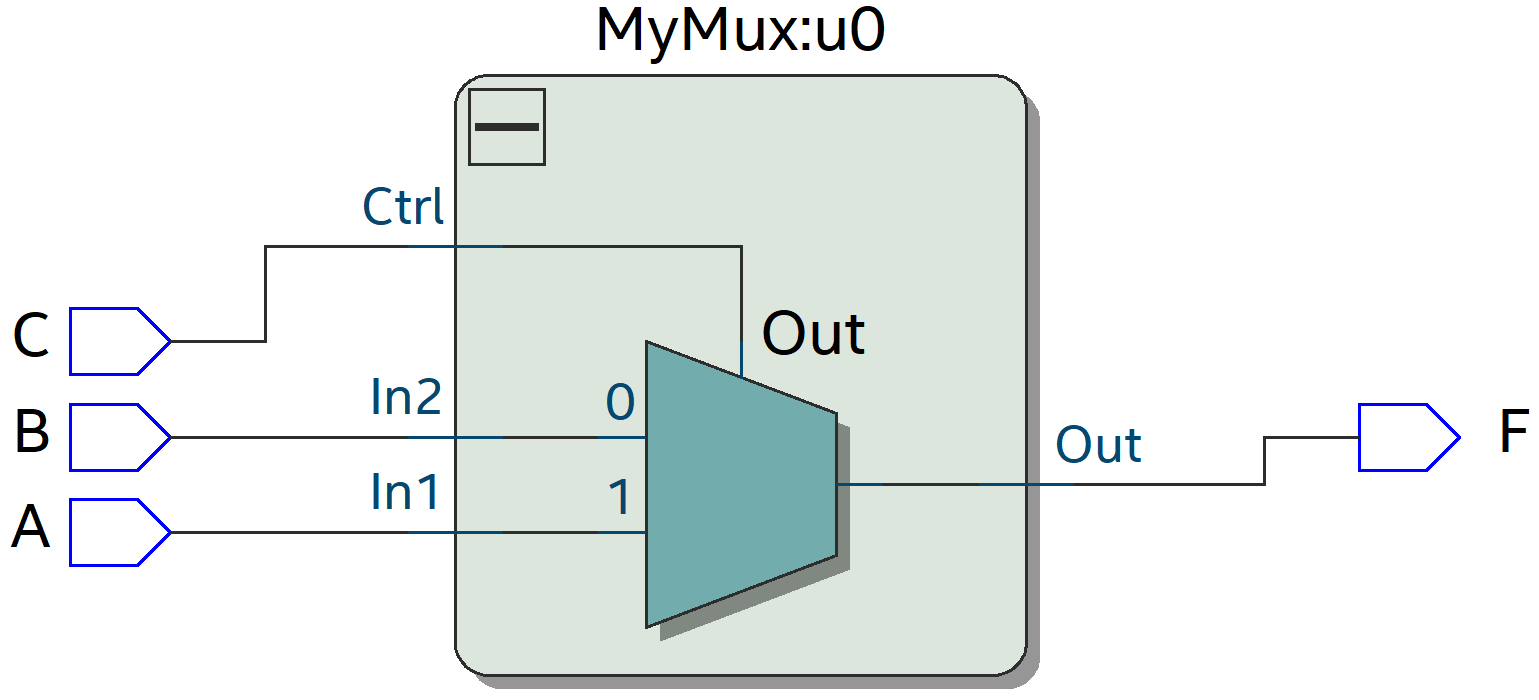
\includegraphics[scale=0.4]{Mux_Structural_Description_RTL2.png}
	\caption{Diagrama RTL del multiplexor, descrito en forma estructural en Verilog (visualización de la instancia interna). \label{fig:mux_str_des_rtl2}}
\end{figure}

\begin{figure}[ht]
	\centering
	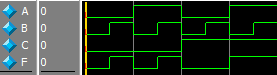
\includegraphics[scale=2]{Mux_Structural_Description_Wave.png}
	\caption{Simulación del multiplexor, descrito en forma estructural en Verilog, con el visor de formas de onda de ModelSim. \label{fig:mux_str_des_wave}}
\end{figure}
	\newpage \section{FSM con flip-flops en estilo \textit{One-Hot} modificado \label{sec:s2}}

\begin{center}
	\begin{minipage}{12cm}
		\begin{tcolorbox}[title=Actividad 2]
			Considerar la tabla ``\textit{ONE – HOT} modificada'':\enter
			
				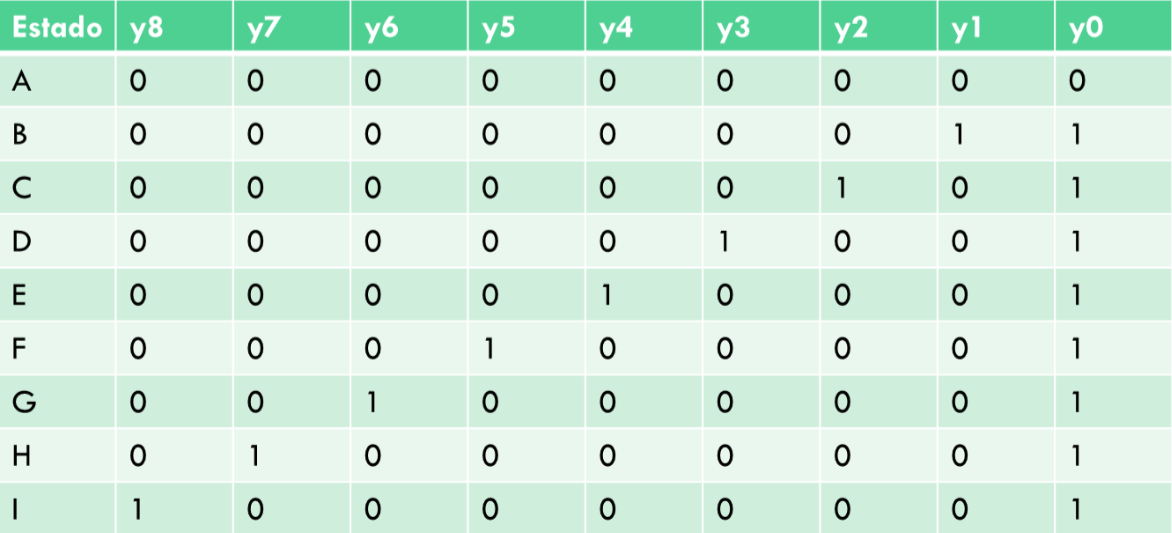
\includegraphics[scale=0.3,center]{OneHotModified.png}
			Diseñar utilizando las ecuaciones de los flip-flops de la tabla modificada. Observar el resultado en el visor RTL. Compilar y simular.
		\end{tcolorbox}	
	\end{minipage}
\end{center}

La visualización RTL de la FSM, descrita en estilo \textit{One-Hot} modificado, se muestra en la \autoref{fig:FSM_OneHotM_RTL}. La implementación en hardware utiliza a los 9 flip-flops descritos en el código y los interconecta de acuerdo a la ecuaciones descritas, haciendo uso de múltiples compuertas lógicas. Las simulaciones se visualizan en la \autoref{fig:FSM_OneHotM_Wave}. Se observa que primero detecta 4 ceros consecutivos y pone en alto a S, aunque W inicia con ``01''. Después de restablecer el sistema (utilizando a RST), la FSM detecta 4 unos consecutivos y pone nuevamente en alto a S, para después volver a ponerla en bajo, ya que la secuencia continúa con ``01''.

En los Anexos se localiza la descripción de la FSM con estilo \textit{One-Hot} modificado. Además de las entradas y salida, se declararon 9 flip-flops y con una lista sensible a los flancos de subida de CLK y de bajada de RST, se describió el comportamiento de cada flip-flop, de acuerdo a su ecuación obtenida. Al momento de restablecer el sistema, se inicializa a cada flip-flop, tomando el estilo \textit{One-Hot} modificado. En comparación con la Actividad 1, el circuito tiene el mismo funcionamiento e implementa la misma cantidad de flip-flops, unicamente cambia el estilo de codificación alterando un poco las ecuaciones del estilo original.

\begin{figure}[ht]
	\centering
	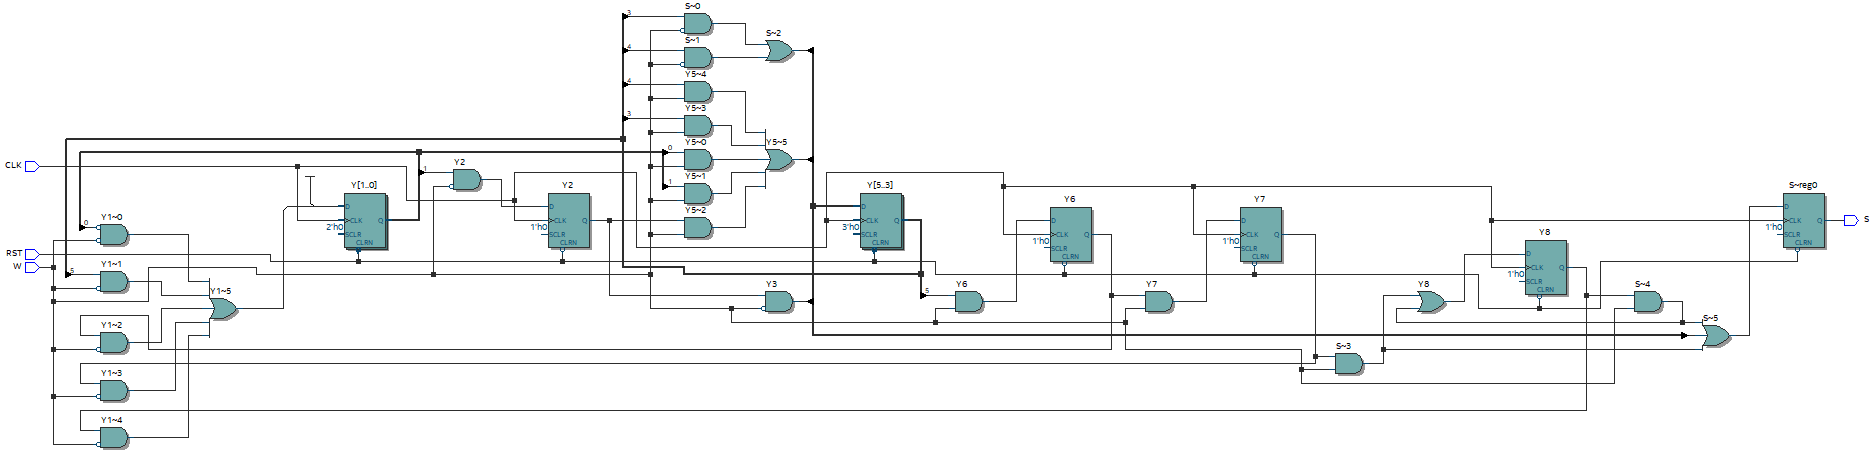
\includegraphics[scale=0.34]{FSM_OneHotM_RTL.png}
	\caption{Diagrama RTL de la FSM, descrita con las ecuaciones de los flip-flops codificados en \textit{One-Hot} modificado. \label{fig:FSM_OneHotM_RTL}}
\end{figure}

\begin{figure}[ht]
	\centering
	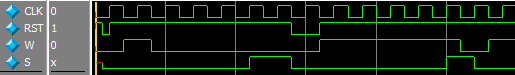
\includegraphics[scale=1.2]{FSM_OneHot_Wave.png}
	\caption{Simulación de la FSM, descrita con las ecuaciones de los flip-flops codificados en \textit{One-Hot} modificado, en el visor de formas de onda de ModelSim. \label{fig:FSM_OneHotM_Wave}}
\end{figure}
	\newpage \section{FSM por comportamiento (estilo \textit{Minimal Bits}) \label{sec:s3}}

\begin{center}
	\begin{minipage}{12cm}
		\begin{tcolorbox}[title=Actividad 3]
			 Describir por comportamiento la FSM del problema que está siendo considerado (como las descripciones vistas en clase). Indicar al compilador usar códigos del registro de estado en forma \textit{``minimal bits''}. Compilar, simular y ver resultado en el visor RTL, ¿se genera el diagrama de estados y la tabla de códigos en los reportes?
			 \enter
			 Para indicar al compilador qué códigos del registro de estado debe usar se debe ir al menú de Quartus correspondiente:\enter
			 
			 $Assignments > Settings > Analysis \& sinthesis > State Machine Processing$
		\end{tcolorbox}	
	\end{minipage}
\end{center}

La visualización RTL de la FSM, descrita por comportamiento en estilo \textit{Minimal Bits}, se muestra en la \autoref{fig:FSM_Behavior_MB_RTL}. En comparación a la Actividad 1 y 2, se implementan solo 2 compuertas lógicas OR, un multiplexor de 4 bits, un selector, un flip-flop D y dos registros de estados. En la \autoref{fig:FSM_Behavior_MB_Graph} se observa el diagrama de estados reportado por el \textit{State Machine Viewer}, que corresponde con el diagrama visto en clase. Además, en la \autoref{fig:FSM_Behavior_MB_Table} se tiene la tabla de códigos utilizada por el software de Quartus, que corresponde al estilo \textit{One-Hot} modificado. Finalmente, en la \autoref{fig:FSM_Behavior_MB_Tran} se hallan todas las transiciones de los estados y que condición se debe dar para hacer el cambio del estado actual al estado destino.

Las simulaciones se visualizan en la \autoref{fig:FSM_Behavior_MB_Wave}. El comportamiento es el mismo que el descrito en actividades anteriores.

En los Anexos se localiza la descripción de la FSM descrita por comportamiento y en estilo \textit{Minimal Bits}. Además de las entradas y salida, se declararon a los 9 estados de la FSM como parámetros, así como dos registros, uno para almacenar el estado actual y otro para el siguiente estado. En una lista sensible se detectan a los flancos de subida de CLK y de bajada de RST y dentro de esta, empleando una estructura \textit{case}, se describió el comportamiento de cada estado y el estado destino de acuerdo al valor de la señal entrada W.

\begin{figure}[ht]
	\centering
	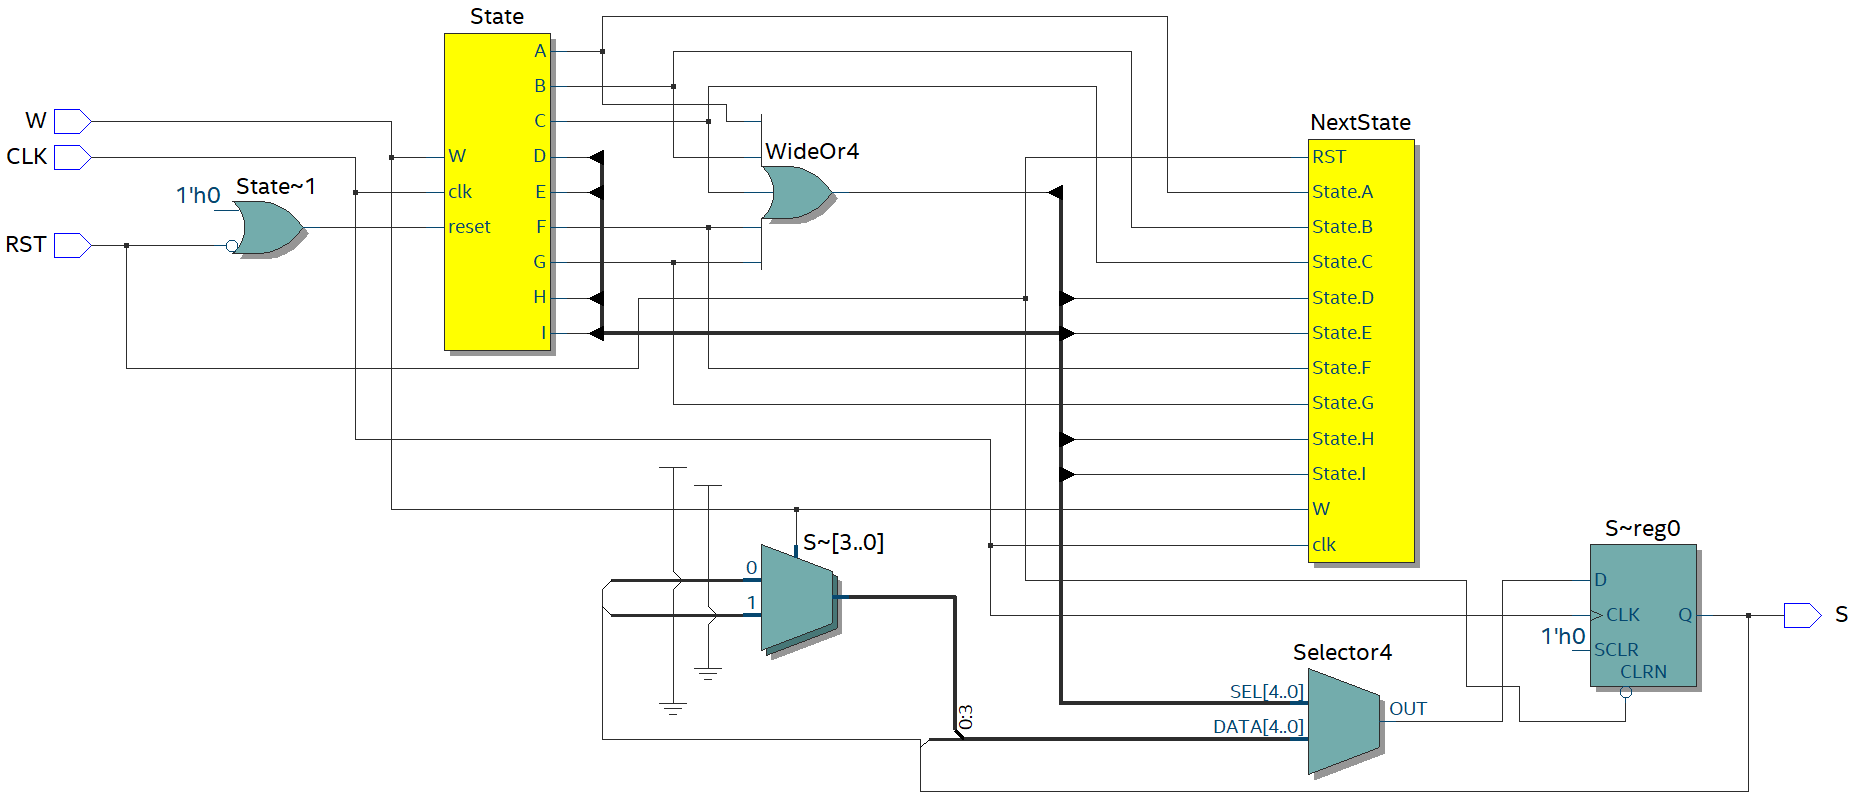
\includegraphics[scale=0.34]{FSM_Behavior_OneHot_RTL.png}
	\caption{Diagrama RTL de la FSM, descrita por comportamiento en codificación \textit{Minimal Bits}. \label{fig:FSM_Behavior_MB_RTL}}
\end{figure}

\begin{figure}[ht]
	\centering
	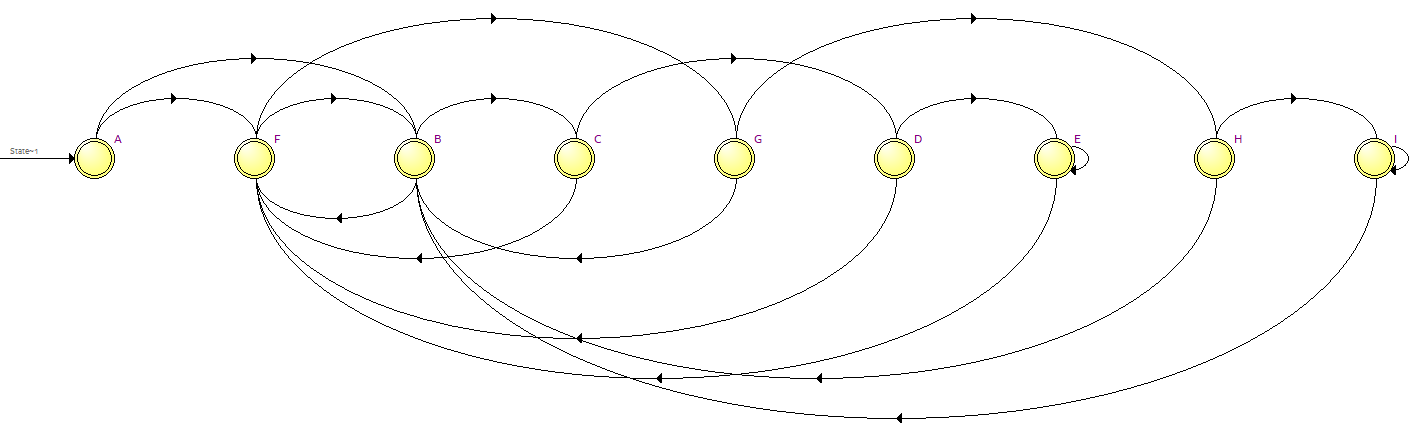
\includegraphics[scale=0.45]{FSM_Behavior_OneHot_Graph.png}
	\caption{Diagrama de estados generado por el \textit{State Machine Viewer} de la FSM estilo \textit{Minimal Bits}. \label{fig:FSM_Behavior_MB_Graph}}
\end{figure}

\begin{figure}[ht]
	\centering
	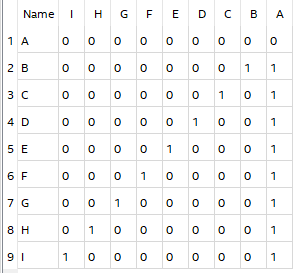
\includegraphics[scale=0.8]{FSM_Behavior_OneHot_Table.png}
	\caption{Tabla de códigos (tipo \textit{One-Hot} modificado) generada por el \textit{State Machine Viewer} de la FSM estilo \textit{Minimal Bits}. \label{fig:FSM_Behavior_MB_Table}}
\end{figure}

\begin{figure}[ht]
	\centering
	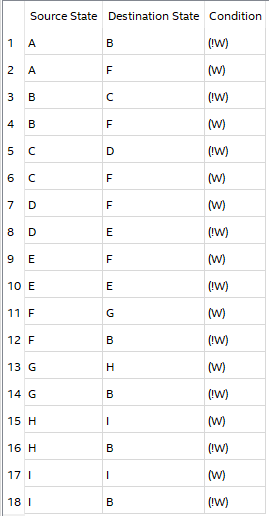
\includegraphics[scale=1.2]{FSM_Behavior_OneHot_Tran.png}
	\caption{Tabla de transiciones generada por el \textit{State Machine Viewer} de la FSM estilo \textit{Minimal Bits}. \label{fig:FSM_Behavior_MB_Tran}}
\end{figure}

\begin{figure}[ht]
	\centering
	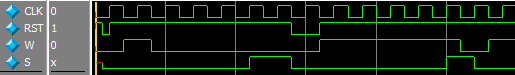
\includegraphics[scale=1.2]{FSM_OneHot_Wave.png}
	\caption{Simulación de la FSM estilo \textit{Minimal Bits}, en el visor de formas de onda de ModelSim. \label{fig:FSM_Behavior_MB_Wave}}
\end{figure}
	%\newpage \section{FSM por comportamiento (estilo \textit{One-Hot}) \label{sec:s4}}

\begin{center}
	\begin{minipage}{12cm}
		\begin{tcolorbox}[title=Actividad 4]
			Repetir el inciso 3 pero indicando codificación \textit{``ONE - HOT''}. ¿Qué códigos \textit{ONE-HOT} fueron utilizados, como los de la tabla normal o la modificada?
		\end{tcolorbox}	
	\end{minipage}
\end{center}

La visualización RTL de la FSM, descrita por comportamiento en estilo \textit{One-Hot}, se muestra en la \autoref{fig:FSM_Behavior_OneHot_RTL}. En comparación a la Actividad 1 y 2, se implementan solo 2 compuertas lógicas OR, un multiplexor de 4 bits, un selector, un flip-flop D y dos registros de estados. En la \autoref{fig:FSM_Behavior_OneHot_Graph} se observa el diagrama de estados reportado por el \textit{State Machine Viewer}, que corresponde con el diagrama visto en clase. Además, en la \autoref{fig:FSM_Behavior_OneHot_Table} se tiene la tabla de códigos utilizada por el software de Quartus, que corresponde al estilo \textit{One-Hot} modificado. Finalmente, en la \autoref{fig:FSM_Behavior_OneHot_Tran} se hallan todas las transiciones de los estados y que condición se debe dar para hacer el cambio del estado actual al estado destino.

Las simulaciones se visualizan en la \autoref{fig:FSM_Behavior_OneHot_Wave}. El comportamiento es el mismo que el descrito en actividades anteriores.

En los Anexos se localiza la descripción de la FSM descrita por comportamiento y en estilo \textit{One-Hot}. La única diferencia de este código con el de la Actividad 3, es el tipo de codificación utilizada en parámetros, ya que se utilizó el \textit{One-Hot}, no obstante, Quartus implementará siempre el estilo \textit{One-Hot} modificado.

\begin{figure}[ht]
	\centering
	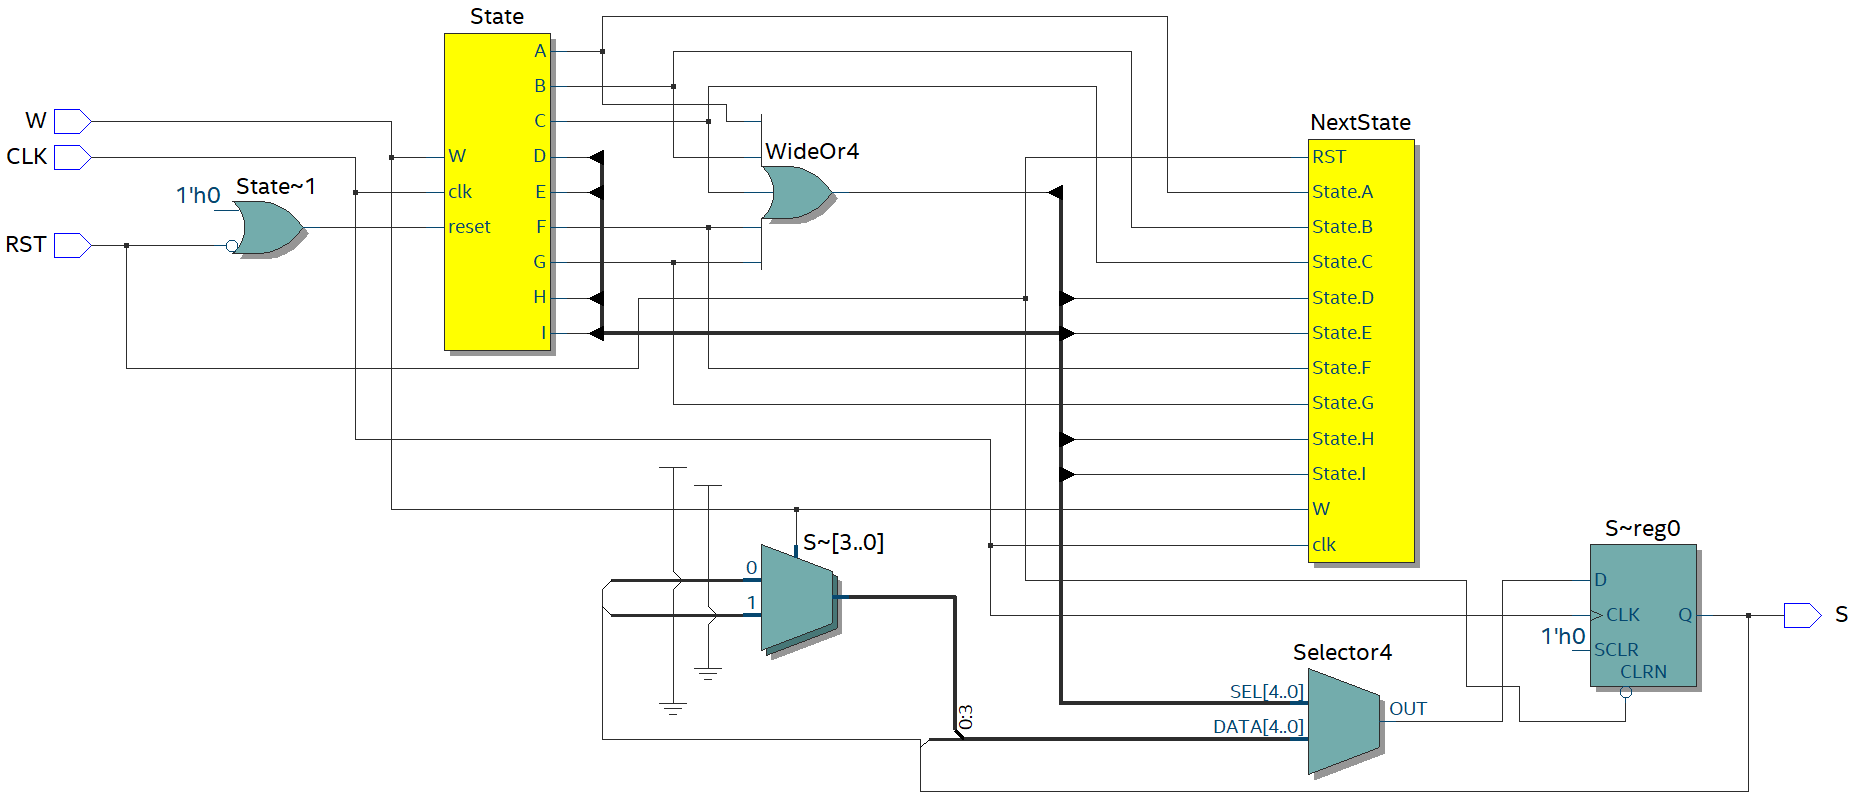
\includegraphics[scale=0.34]{FSM_Behavior_OneHot_RTL.png}
	\caption{Diagrama RTL de la FSM, descrita por comportamiento en codificación \textit{One-Hot}. \label{fig:FSM_Behavior_OneHot_RTL}}
\end{figure}

\begin{figure}[ht]
	\centering
	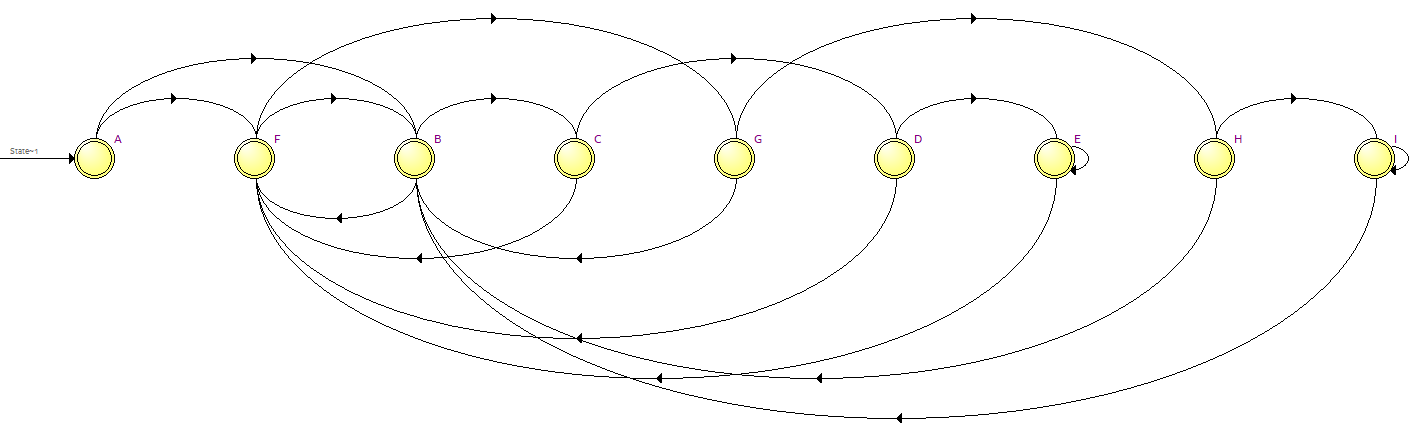
\includegraphics[scale=0.45]{FSM_Behavior_OneHot_Graph.png}
	\caption{Diagrama de estados generado por el \textit{State Machine Viewer} de la FSM estilo \textit{One-Hot}. \label{fig:FSM_Behavior_OneHot_Graph}}
\end{figure}

\begin{figure}[ht]
	\centering
	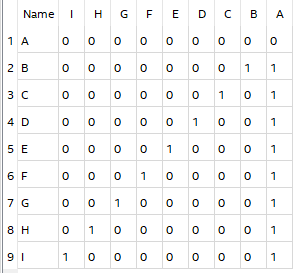
\includegraphics[scale=0.8]{FSM_Behavior_OneHot_Table.png}
	\caption{Tabla de códigos (tipo \textit{One-Hot} modificado) generada por el \textit{State Machine Viewer} de la FSM estilo \textit{One-Hot}. \label{fig:FSM_Behavior_OneHot_Table}}
\end{figure}

\begin{figure}[ht]
	\centering
	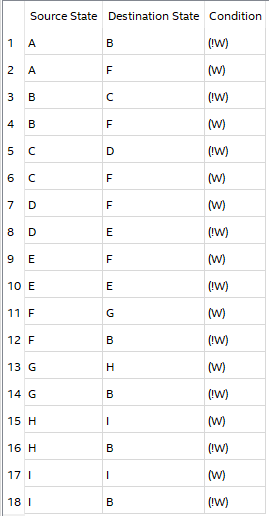
\includegraphics[scale=1.2]{FSM_Behavior_OneHot_Tran.png}
	\caption{Tabla de transiciones generada por el \textit{State Machine Viewer} de la FSM estilo \textit{One-Hot}. \label{fig:FSM_Behavior_OneHot_Tran}}
\end{figure}

\begin{figure}[ht]
	\centering
	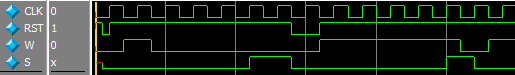
\includegraphics[scale=1.2]{FSM_OneHot_Wave.png}
	\caption{Simulación de la FSM estilo \textit{One-Hot}, en el visor de formas de onda de ModelSim. \label{fig:FSM_Behavior_OneHot_Wave}}
\end{figure}

	
	\newpage
	\section{Conclusiones}
	Se logró detectar secuencias de unos y ceros describiendo una máquina de estados finitos de diferentes maneras.
	
	\enter
	
	Se implementó una máquina de estados utilizando las ecuaciones de cada estado para la detección de secuencias y variando el uso de tabla \textit{one hot} y
	\textit{one hot} modificada, analizando los resultados del diagrama RTL.
	
	\enter
	
	Se implementó una máquina de estados finitos por comportamiento, variando el uso del código \textit{minimal bits} y \textit{one hot}, analizando el reporte en su configuración de máquina de estados finitos, comprobando la diferencia que hace el compilador para implementar \textit{minimal bits} o \textit{one hot}.
	
	\enter
	
	Se implementó la detección de secuencia de bit utilizando corrimientos lógicos y aritméticos con 2 y 1 registros, respectivamente. Se encontraron maneras alternativas de resolver el problema de la máquina de estados finitos sin usar tablas de codificación definidas.
	
	\newpage \section{Anexos}

\subsection{Descripciones del hardware}

\lstinputlisting[
	language=verilog,
	label=prog:mux_str_des,
	caption={Descripción en Verilog del multiplexor en forma estructural.}
]{
	../../Proyectos/Mux_Structural_Description/Mux_Structural_Description.v
}

\lstinputlisting[
language=verilog,
label=prog:mux_ip_catalog,
caption={Descripción en Verilog del multiplexor en forma estructural, instanciando un archivo creado con IP Catalog.}
]{
	../../Proyectos/Mux_IP_Catalog/Mux_IP_Catalog.v
}

\subsection{Bancos de pruebas (\textit{Test Benches})}

\lstinputlisting[
	language=verilog,
	%label=prog:asign,
	caption={Banco de prueba para el \autoref{prog:mux_str_des}.}
]{
	../../Proyectos/Mux_Structural_Description/simulation/modelsim/Mux_Structural_Description.vt
}


\lstinputlisting[
language=verilog,
%label=prog:asign,
caption={Banco de prueba para el \autoref{prog:mux_ip_catalog}.}
]{
	../../Proyectos/Mux_IP_Catalog/simulation/modelsim/Mux_IP_Catalog.vt
}
\end{document}


